\documentclass[11pt,a4paper,oneside,twocolumn]{article}
%\usepackage{fourier} %fonte plus lisible
\usepackage{hyperref}
\usepackage[T1]{fontenc}
\usepackage[francais]{babel}
\usepackage[utf8]{inputenc}
\usepackage{cite}
%\usepackage{lipsum}
\usepackage{amsmath}
\usepackage{amsthm}
\usepackage{amssymb}
\usepackage{verbatim}
%\usepackage{varwidth}
\usepackage{tikz}
\usetikzlibrary{babel}
\usepackage{url}
\usepackage{subcaption}
\usepackage[siunitx]{circuitikz}
\usepackage{siunitx}
\usepackage{listings}
\usepackage{caption}
\DeclareCaptionType{equ}[\textsc{Équation}]{}

\title{Utiliser des LEDs sur Arduino}
\author{Guillaume \textsc{Huysmans}, Miika \textsc{Lehtonen}}
\hypersetup{pdfauthor={Guillaume Huysmans, Miika Lehtonen},
	pdftitle={Utiliser des LEDs sur Arduino},
	pdfsubject={électronique, circuit, diode},
	pdfkeywords={électronique, physique, circuit, diode}}

\begin{document}
\maketitle

\section{Un peu de physique}
Avant de construire un circuit avec un Arduino, nous allons d'abord comprendre
comment en faire un sans. L'Arduino nous permettra ensuite de \emph{programmer}
facilement des comportements plus complexes.

\subsection{Ampoule}
Une ampoule classique est constituée de trois éléments principaux :
un \textbf{culot} (la partie métallique qui se visse dans une douille), une
\textbf{ampoule} de verre à l'intérieur de laquelle se trouve un gaz
rare\footnote{Les gaz rares se trouvent dans la colonne de l'hélium dans le
tableau périodique.},
%FIXME lequel ?
qui permet au dernier élément, un \textbf{filament} en
tungstène\footnote{W dans le tableau périodique des éléments.},
de chauffer assez fort pour émettre de la lumière lorsqu'il est traversé par un
courant.

Le circuit électrique le plus simple qu'on peut imaginer est celui constitué
d'une ampoule et d'une pile (voir figure \ref{fig:lb}).

\begin{figure}[ht]
	\centering
	\begin{circuitikz}
		\draw (0,0)
			to[battery,i=+] ++(2,0) to ++(0,-1.5)
			to[lamp] ++(-2,0) to ++(0,1.5);
	\end{circuitikz}
	\caption{Montage avec une ampoule}
	\label{fig:lb}
\end{figure}

Le filament de l'ampoule (voir figure \ref{fig:micro}) \textbf{résiste} au
passage du courant, ce qui le fait chauffer (par effet Joule) et émettre de la
lumière (voir figure \ref{fig:w}).
%(par convention
%\footnote{Cette convention s'est avérée fausse...}, en partant du +)

\begin{figure}[ht]
	\centering
	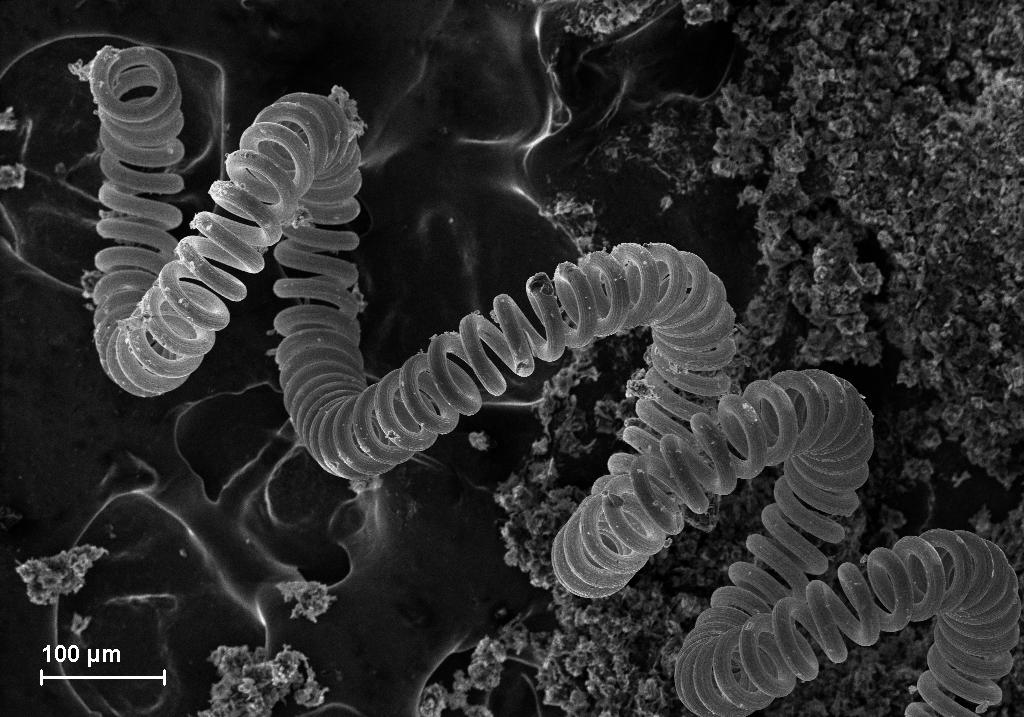
\includegraphics[width=\linewidth]{w.jpg}
	\caption{Filament vu au microscope électronique (source : Wikipédia)}
	\label{fig:micro}
\end{figure}

\begin{figure}[ht]
	\centering
	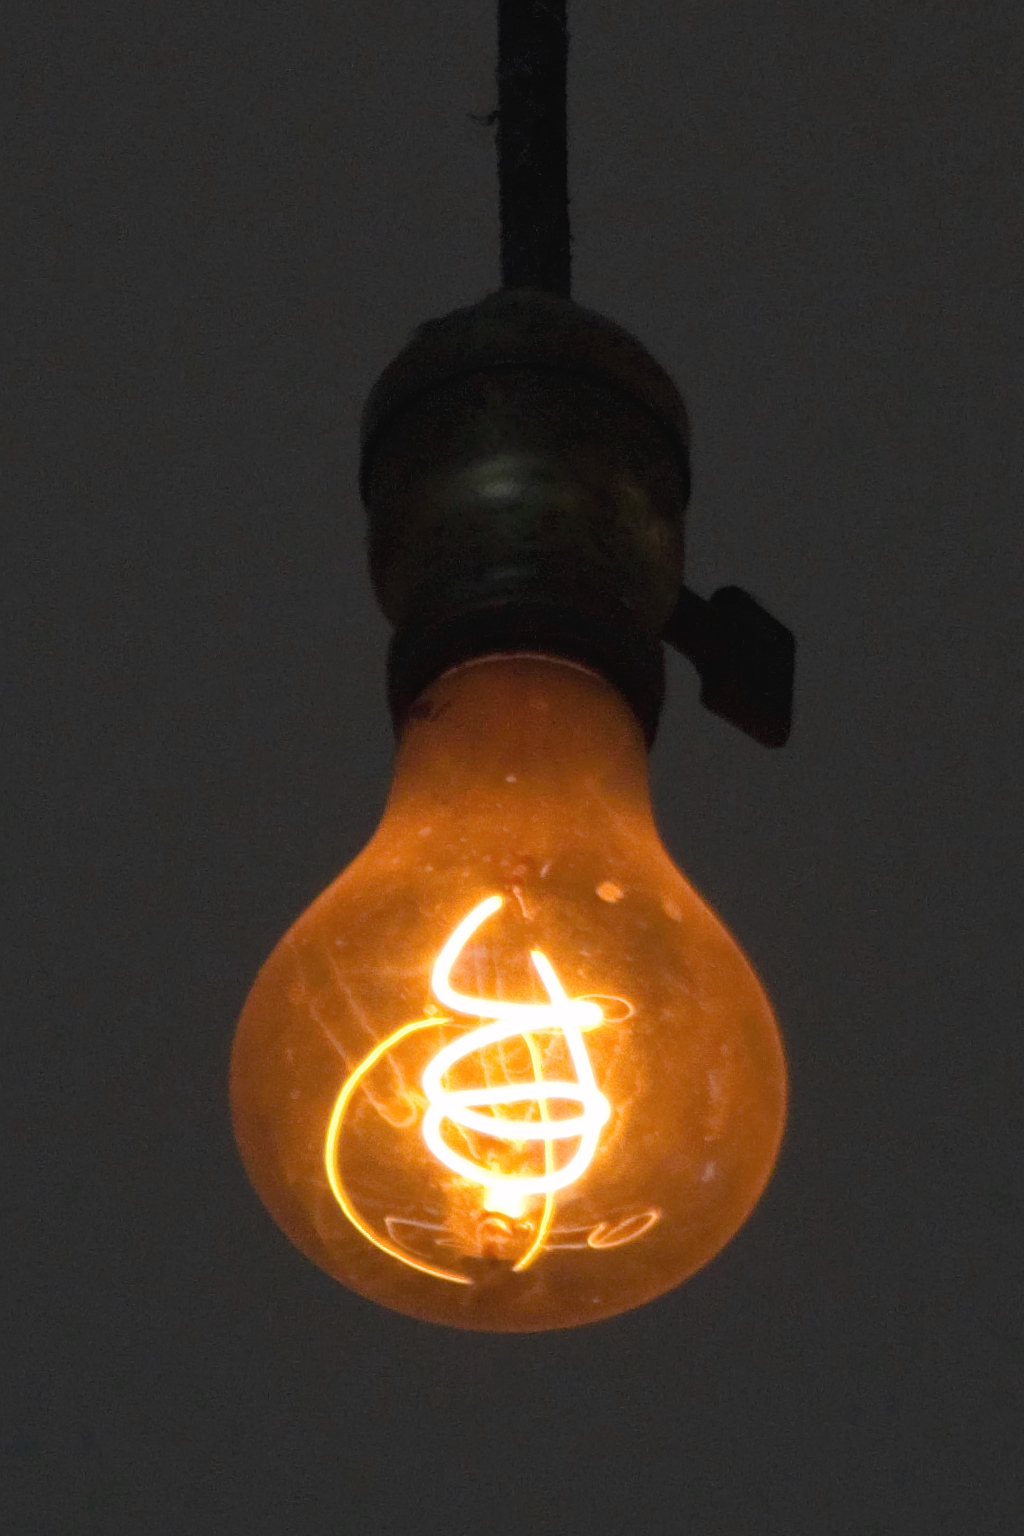
\includegraphics[width=0.5\linewidth]{centenaire.jpg}
	\caption{Ampoule centenaire (Wikipédia)}
	\label{fig:w}
\end{figure}

Le même schéma s'applique dans une maison mais comme la puissance est bien
supérieure, il faut des câbles plus épais (cf. équation \ref{eqn:pouillet}) si
on ne veut pas qu'ils chauffent.
Dans nos ateliers, nous ne toucherons pas à ça, c'est bien trop dangereux.

\begin{equ}[ht]
	\begin{equation*}
		R=\frac{\rho\times l}s
	\end{equation*}
	%\[
	%\begin{array}{ll}
		%R = \frac{\rho\times l}s \quad \text{où} & bidule \\
		%& 42
	%\end{array}
	%\]
	\caption{Loi de Pouillet, où $R$ est la résistance, $\rho$ la résistivité
	du matériau (qu'on trouve dans des tables), $l$ la longueur du fil (en
	mètres) et $s$, sa section (en $\text{m}^2$).}
	%FIXME vérifier que c'est pas des mm, on sait jamais
	\label{eqn:pouillet}
\end{equ}

Le problème, c'est que les pertes en chaleur sont importantes\footnote{Sur
Wikipédia, on parle de moins de 5\% de rendement : le reste de l'énergie ne
sert pas à éclairer.} (avez-vous déjà touché une ampoule allumée depuis des
heures ?); c'est la raison pour laquelle on commence à les voir disparaître de
nos maisons au profit des LEDs
(diodes électroluminescentes\footnote{\emph{Light-Emitting Diode} en anglais})

\subsection{LED}
Une LED émet aussi de la lumière quand elle est traversée par un courant mais
contrairement à une ampoule, elle ne se comporte pas comme une résistance (voir
figures \ref{fig:ohm} et \ref{fig:diode}).

%Pour calculer la valeur de cette résistance, nous allons combiner quatre choses :
Aux bornes d'une diode, il y a une chute de tension puisqu'elle ne conduit pas
en dessous de sa tension de seuil $V_F$ (voir figure \ref{fig:diode}).
Pour une diode rouge :
\begin{equation}
	V_F=1.7\si{V}
\end{equation}

Cette valeur dépend de la longueur d'onde (voir figure \ref{fig:wave}) de la
lumière émise, c'est ce qu'exprime la relation de Planck-Einstein\footnote{Ces
scientifiques seront récompensés par deux prix Nobel de physique, le premier en
1918 et le second, en 1921.} :
\begin{equation}
	E=hf=\frac h\lambda
\end{equation}
$h$ est la constante de Planck :
\begin{equation}
h\approx6.63\times10^{-34}\si{J.s}
\end{equation}

\begin{figure}[ht]
	\centering
	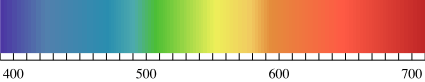
\includegraphics[width=\linewidth]{visible.png}
	\caption{Spectre visible selon la longueur d'onde ($\lambda$) en nanomètres}
	\label{fig:wave}
\end{figure}

La tension de seuil se calcule comme suit :
\begin{equation}\label{eq:led}
E=e\times V_F \iff V_F=\frac Ee
\end{equation}
$e$ est la charge d'un électron :
\begin{equation}
e\approx-1.602\times10^{-19}\si{A.s^{-1}}
\end{equation}
%FIXME faire le calcul pour voir si c'est correct...

\begin{figure}[ht]
	\centering
	\begin{tikzpicture}
		\draw[->] (0,0) -- (0,3) node[above] {$I$};
		\draw[->] (0,0) -- (3,0) node[right] {$U$};
		\draw[domain=0:3,variable=\x] plot({\x,\x});
	\end{tikzpicture}
	\caption{Loi d'Ohm \eqref{eq:ohm}}
	\label{fig:ohm}
\end{figure}

\begin{figure}[ht]
	\centering
	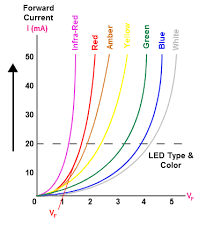
\includegraphics[width=0.4\textwidth]{lediv.png}
	\caption{Caractéristiques de différentes diodes
		(source : forum All About Circuits)}
	\label{fig:diode}
\end{figure}

Pour éviter un court-circuit qui grillerait la diode avec trop de courant, il
faut soi-même ajouter une résistance (voir figure \ref{fig:led}).

\begin{figure}[ht]
	\centering
	\begin{circuitikz}
		\draw (0,0)
			to[battery,v=U] ++(2,0)
			to[R=R] ++(0,-2)
			to[leD,invert] ++(-2,0)
			to ++(0,2);
	\end{circuitikz}
	\caption{Montage avec une LED}
	\label{fig:led}
\end{figure}

Le courant maximal toléré par nos LEDs rouges est indiqué dans leur
datasheet\footnote{%Il n'est pas toujours facile de les retrouver, surtout quand
%on commande directement sur des sites chinois. Voici quand même un exemple de
Par exemple : \url{https://www.vishay.com/docs/83171/tlur640.pdf}.}.
\begin{equation}
	I_L=20\si{mA}
\end{equation}

Le courant $I_R$ qui traverse une résistance de valeur $R$ est proportionnel à
la tension $U_R$ à ses bornes. Voici l'équation de la loi d'Ohm déjà illustrée à
la figure \ref{fig:ohm} :
\begin{equation}\label{eq:ohm}
	U_R=R\times I_R
	\iff R=\frac{U_R}{I_R}
\end{equation}

Des composants en série sont traversés par le même courant :
\begin{equation}
	I_L=I_R
\end{equation}
Pour vous en convaincre, essayez de reproduire le montage illustré à la
figure \ref{fig:ser} !
%FIXME plus facile avec la loi des mailles ?
%\footnote{C'est une des conséquences des lois de Kirchoff.}.

\begin{figure}[ht]
	\centering
	\begin{circuitikz}
		\draw (0,0)
			to[battery] ++(0,2)
			to[R=R] ++(2,0)
			to[ammeter] ++(1,0)
			to[R=R] ++(2,0)
			to[ammeter] ++(0,-2)
			to ++(-5,0);
	\end{circuitikz}
	\caption{Résistances en série}
	\label{fig:ser}
\end{figure}

Voici donc comment calculer la valeur de la résistance à placer avant ou après
la LED :
\begin{equation}
	R=\frac{U-V_F}{I_L}
\end{equation}
avec $U$, la tension d'alimentation du circuit.

\section{Arduino}
Un microcontrôleur est un petit ordinateur doté d'entrées-sorties. Il peut
contrôler d'autres équipements (moteurs, écrans...) et recevoir des données
provenant de capteurs (température, humidité, pression, luminosité...). Dans
nos ateliers, nous utiliserons des ESP32 compatibles avec la plateforme Arduino.

\subsection{Installation}
L'environnement de développement intégré
(IDE\footnote{\emph{Integrated Development Environment} en anglais})
est disponible gratuitement
en ligne\footnote{\url{https://www.arduino.cc/en/Main/Software}}.
Une fois téléchargé, il faut installer une carte supplémentaire en passant par
le \emph{Board Manager} (voir figure \ref{fig:boardman}) et la sélectionner
dans le menu (voir figure \ref{fig:boardmenu}).

\begin{figure}[ht]
	\centering
	%FIXME
	%\includegraphics[width=0.8\linewidth]{boardmanager.png}
	\caption{Arduino Board Manager}
	\label{fig:boardman}
\end{figure}

\begin{figure}[ht]
	\centering
	%FIXME
	%\includegraphics[width=0.8\linewidth]{boardmenu.png}
	\caption{Cartes compatibles Arduino}
	\label{fig:boardmenu}
\end{figure}

\subsection{Branchements}
Ici, il n'est pas nécessaire de passer par une étape de contrôle : on peut
directement alimenter la diode avec une
GPIO\footnote{\emph{General Purpose Input/Output} en anglais}, voir figure
\ref{fig:ardled}.

\begin{figure}[ht]
	\centering
	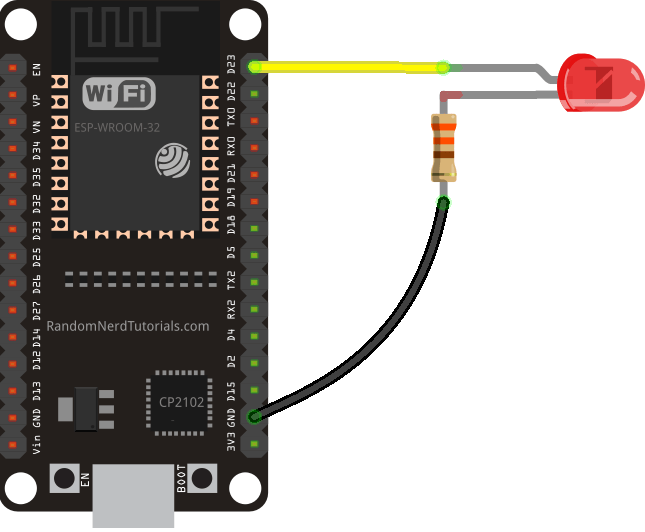
\includegraphics[width=\linewidth]{esp32-led.png}
	\caption{LED branchée à un ESP32}
	\label{fig:ardled}
\end{figure}

Par contre, il est \textbf{indispensable} d'utiliser une résistance pour limiter
le courant qui y circule sous peine de le faire griller.
La figure \ref{fig:arduinoshort} montre en gras un court-circuit sur le schéma
d'un Arduino original.

La datasheet de
l'ESP32\footnote{\url{https://www.espressif.com/sites/default/files/documentation/esp32\_datasheet\_en.pdf},
section 5.3} indique deux valeurs intéressantes à propos des sorties:
\begin{itemize}
\item le courant maximal :
	\begin{equation}
		I_{OH}=20\si{mA}
	\end{equation}
\item la tension minimale :
	\begin{equation}
		V_{OH}=2.64\si{V}
	\end{equation}
\end{itemize}

\begin{figure}[ht]
	\centering
	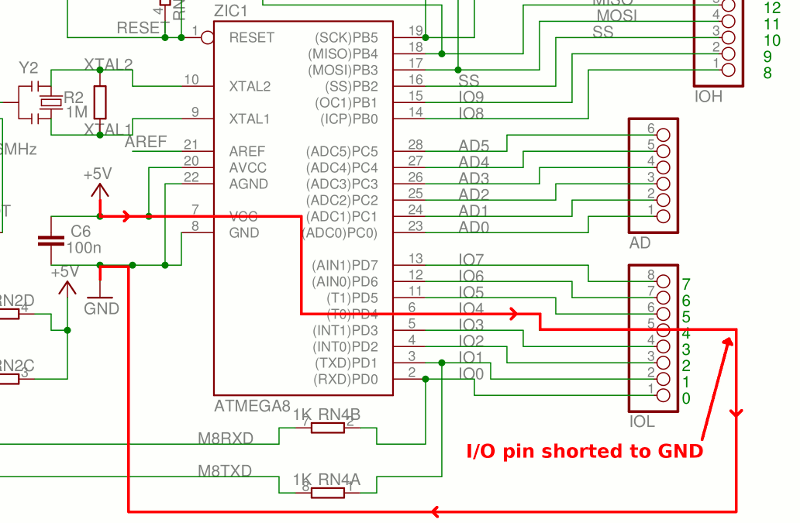
\includegraphics[width=\linewidth]{arduinoshort.png}
	\caption{Court-circuit dans un Arduino (source :
	\href{https://www.rugged-circuits.com/10-ways-to-destroy-an-arduino}
	{\emph{10 ways to destroy an Arduino}})}
	\label{fig:arduinoshort}
\end{figure}

%FIXME pas utile vu que c'est mal espacé et mal placé :/
\newcommand\esymbol[1]{\begin{circuitikz}
\draw (0,0) to [#1] (1,0); \end{circuitikz}}

Pour éviter de représenter la carte toute entière sur le schéma, nous
utiliserons des symboles supplémentaires pour
la masse commune et
les GPIOs (voir figure \ref{fig:gpio}).

\begin{figure}[ht]
	\centering
	\begin{circuitikz}
		\draw[o-] (0,0) node[left]{GPIO} -- (1,0);
		\draw (1,0) to[leD] ++(2,0) to[R=$R$] ++(0,-2) node[ground]{};
	\end{circuitikz}
	\caption{LED branchée à une GPIO}
	\label{fig:gpio}
\end{figure}

Vérifions la valeur de la résistance utilisée à la figure \ref{fig:gpio}. La
figure \ref{fig:res} nous permet de trouver que $R=330\Omega$. En appliquant
\eqref{eq:led} avec $U=V_{OH}$, on trouve :
\begin{equation*}
	I_L=\frac{U-V_F}R=\frac{2.64-1.5}{330}=3.45\si{mA}<I_{OH}
\end{equation*}

\begin{figure}[ht]
	\centering
	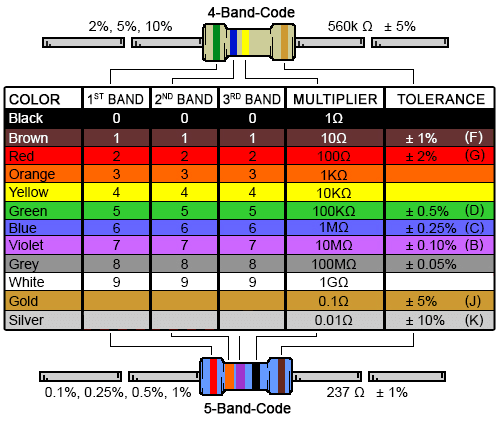
\includegraphics[width=\linewidth]{resistor-color-chart.png}
	\caption{Codes couleurs des résistances (source :
	\href{https://www.digikey.be/fr/resources/conversion-calculators/conversion-calculator-resistor-color-code-4-band}{Digikey})}
	\label{fig:res}
\end{figure}

\subsection{Programmation}
L'environnement Arduino se programme en <<~C++ simplifié~>>.
%Nous n'utiliserons qu'une infime partie de ce langage.
Tout est fait pour qu'on puisse s'inspirer d'exemples existants :

\begin{lstlisting}[frame=single,language=C++,caption=
Exemple : \texttt{01.Basics/Blink}]
int led = 13;

void setup() {
  pinMode(led, OUTPUT);
}

void loop() {
  digitalWrite(led, HIGH);
  delay(1000);

  digitalWrite(led, LOW);
  delay(1000);
}
\end{lstlisting}

À la première ligne, \texttt{led} est définie comme une variable entière
(\texttt{int}) initialisée à la valeur 13. De cette façon, si on choisit plus
tard d'utiliser une autre sortie, il ne faudra modifier que cette déclaration.

Ensuite, la fonction \texttt{setup} est définie, elle ne prend aucun argument
(il n'y a rien entre parenthèses). La
documentation\footnote{\url{https://www.arduino.cc/reference/en/language/structure/sketch/setup/}}
indique que cette fonction sera appelée une seule fois par l'environnement
Arduino, au démarrage au programme. Dans ce programme, \texttt{setup} appelle
seulement
\texttt{pinMode}\footnote{\url{https://www.arduino.cc/reference/en/language/functions/digital-io/pinmode/}}
qui va configurer l'entrée-sortie \texttt{led} dans un mode passé comme second
paramètre : entrée (\texttt{INPUT}), sortie (\texttt{OUTPUT}) ou encore une
entrée avec une résistance de tirage (\texttt{INPUT\_PULLUP}) qui nous sera
utile avec des boutons.

Enfin, on définit \texttt{loop}, la fonction qui sera appelée continuellement
après \texttt{setup}. À l'intérieur, on voit deux bouts de code très semblables
qui changent l'état de la sortie puis attendent une seconde (quelle est l'unité
de temps utilisée par \texttt{delay}, d'ailleurs ?).

L'environnement Arduino est bien documenté : cliquez droit sur un identificateur
(\texttt{digitalWrite}, \texttt{delay}...) à propos duquel vous voulez vous
renseigner puis cliquez sur \emph{Find in Reference} pour voir la page de
documentation qui lui est associée.
Une page\footnote{\url{https://www.arduino.cc/reference/en/}} reprend aussi la
liste des fonctions disponibles.

\subsection{L'art du clignotement}
Généralisons l'exemple donné précédemment en nommant $a$ et $b$ les délais dans
\texttt{loop}. La figure \ref{fig:slice} montre un cycle complet.

\begin{figure}[ht]
	\centering
	%TODO convertir encodage différentiel en graphe ? bof, dépend qd mm
	\begin{tikzpicture}
		\draw
			(0,1) to ++(1,0)
			to ++(0,-1) to ++(1,0);
		\draw[<->] (0,-0.5) -- node[below]{$a$} ++(1,0);
		\draw[<->] (1,-0.5) -- node[below]{$b$} ++(1,0);
	\end{tikzpicture}
	\caption{Cycle de clignotement}
	\label{fig:slice}
\end{figure}

Le cycle se répète à cette fréquence :
\begin{equation}
	f=\frac1{a+b}
\end{equation}

Le rapport cyclique\footnote{\emph{duty cycle} en anglais} est la proportion du
temps pendant lequel la diode est allumée :
\begin{equation}
	\alpha=\frac a{a+b}=a\times f
\end{equation}

Pour voir si vous avez bien compris le principe, essayez de répondre à ces
questions :
\begin{enumerate}
\item Comment doubler $f$ en préservant $\alpha$ ?
\item En augmentant $f$, que se passe-t-il <<~à la limite~>> ? Que fait la
	diode ? Pouvons-nous faire confiance à nos yeux ?
\item Est-ce que le code fonctionnerait encore avec un seul \texttt{delay} ?
	Pourquoi ?
\item Comment contrôler deux sorties à la fois ?
\end{enumerate}

\end{document}
